% !TEX program = pdflatex
% ============================================================================
% CtxVigil — DA2 Project Review Report (IEEE conference format)
%
% Compile on Overleaf:
%   1. Upload the entire `report/` folder (this file + figures/) as a project.
%   2. Set the compiler to pdfLaTeX (Menu -> Compiler -> pdfLaTeX).
%   3. Recompile. No bibliography step is needed (references are inline).
%
% TODO for the authors (title block): fill in Saumya's full name, roll
% numbers, department, institution, and guide name where marked with % TODO.
% ============================================================================
\documentclass[conference]{IEEEtran}
\usepackage{graphicx}
\usepackage{amsmath}
\usepackage{amssymb}
\usepackage{booktabs}
\usepackage{array}

\graphicspath{{figures/}}

\begin{document}

\title{CtxVigil: An Explainable Multi-View Protection Layer Against
Indirect Prompt Injection in LLM Web Agents}

\author{\IEEEauthorblockN{Rishabh Tripathi\IEEEauthorrefmark{1}
\and Saumya\IEEEauthorrefmark{2}} % TODO: Saumya's full name
\IEEEauthorblockA{\IEEEauthorrefmark{1}Roll No.\ 24BRS1136 \quad
\IEEEauthorrefmark{2}Roll No.\ 24BRS1065
\\ Department of Computer Science and Engineering
% TODO: institution name
\\ Course: BCSE306L -- Artificial Intelligence (Final Project \& Viva Evaluation)
\\ \texttt{rishabh.j.tripathi2903@gmail.com}} % TODO: second author's e-mail
}

\maketitle

\begin{abstract}
Large language model (LLM) web agents read untrusted web content and take
actions on the user's behalf, which exposes them to \emph{indirect prompt
injection}: attacker-authored text, hidden in a page's visible text, DOM,
HTML comments, or accessibility tree, that instructs the agent to abandon its
task and perform a harmful action. This paper presents CtxVigil, a protection
layer that sits between an agent and the web and combines three complementary
components: (i) a deterministic, explainable scan pipeline that normalises a
page into four content views, runs seven rule detectors, and maps a weighted
0--100 risk score to \texttt{allow}/\texttt{sanitize}/\texttt{confirm}/
\texttt{block} verdicts with withheld-content containment; (ii) an independent
action gate that blocks or escalates tool actions using task alignment,
risk-category postures, and scan evidence; and (iii) a dual-head multi-view
fusion network over MiniLM sentence embeddings of four agent-context views
(user task, system prompt, proposed action, observation) plus a DeBERTa-v3
prompt-injection classifier. On a 20{,}000-sample benchmark curated from
InjecAgent- and BIPIA-style scenarios with hard negatives, the fine-tuned
DeBERTa-v3-small classifier reaches 100.00\% accuracy, precision, recall, and
F1 (ROC-AUC 1.000) on the 3{,}000-sample held-out test set; the fusion network
reaches 100\% F1 on 1{,}000 hold-out episodes. The rule-based layer passes all
seven contract fixtures and all six live agent episodes, including a
hidden-ARIA injection that a sighted reviewer cannot see, at 2--21\,ms per
episode on a commodity CPU, fully offline and fail-closed.
\end{abstract}

\begin{IEEEkeywords}
indirect prompt injection, LLM agents, action gate, multi-view fusion,
DeBERTa-v3, uncertainty estimation, web security
\end{IEEEkeywords}

\section{Introduction}
Autonomous LLM web agents navigate external environments---product pages,
support portals, and admin dashboards---and act on what they read. Because the
agent's prompt is assembled at runtime from untrusted page content, any third
party who controls a web page can inject instructions into the agent's
context. Indirect prompt injection has been shown to hijack agents into
exfiltrating data, changing account settings, or executing fraudulent
transactions~\cite{greshake2023,injecagent2024,bipia2023}, and it is listed
among the top risks for LLM-integrated applications~\cite{owasp2025}.

Three observations motivate CtxVigil. First, \emph{a single view is not
enough}: an injection can be invisible on screen (a hidden DOM span, an HTML
comment, an \texttt{aria-label} payload aimed at the accessibility tree), so
protection must reconcile the same page across multiple representations.
Second, \emph{an opaque score is not enough}: a verdict that cannot cite the
view, the signal, and the offending span is weak evidence for a user or an
auditor. Third, \emph{blocking everything is not protection}: imperative
phrasing occurs in benign controls (``Click here to submit''), so a usable
layer must verify task alignment rather than flag every command-like string.

CtxVigil therefore couples a transparent, rule-based scan-and-gate layer
(the deployable product, distributed as the \texttt{ctxvigil} npm SDK) with a
learned multi-view fusion network (the DA-1 model component). The
contributions of this paper are:

\begin{itemize}
\item A four-view page normalisation (visible text, rendered DOM, hidden DOM,
accessibility tree) with concealment metadata, feeding seven deterministic
detectors whose findings carry view, selector, signals, and score
contribution (Section~\ref{sec:methodology}).
\item An independent action gate that treats \emph{what the agent does} as a
separate decision from \emph{what the agent read}, combining task alignment,
risk-category postures, and finding triggers---so a page that scans clean can
still have its unrelated account change blocked.
\item A multi-view fusion and uncertainty network over 384-d MiniLM
embeddings of four agent-context views plus the DeBERTa injection probability,
trained with a dual risk/uncertainty objective (Sections~\ref{sec:fusion}
and~\ref{sec:results-ml}).
\item An evaluation on a 20{,}000-sample benchmark, 5{,}000 synthetic
multi-view episodes, seven contract fixtures, and six live agent episodes,
with latency measurements on commodity CPU (Section~\ref{sec:results}).
\end{itemize}

\begin{figure*}[t]
\centering
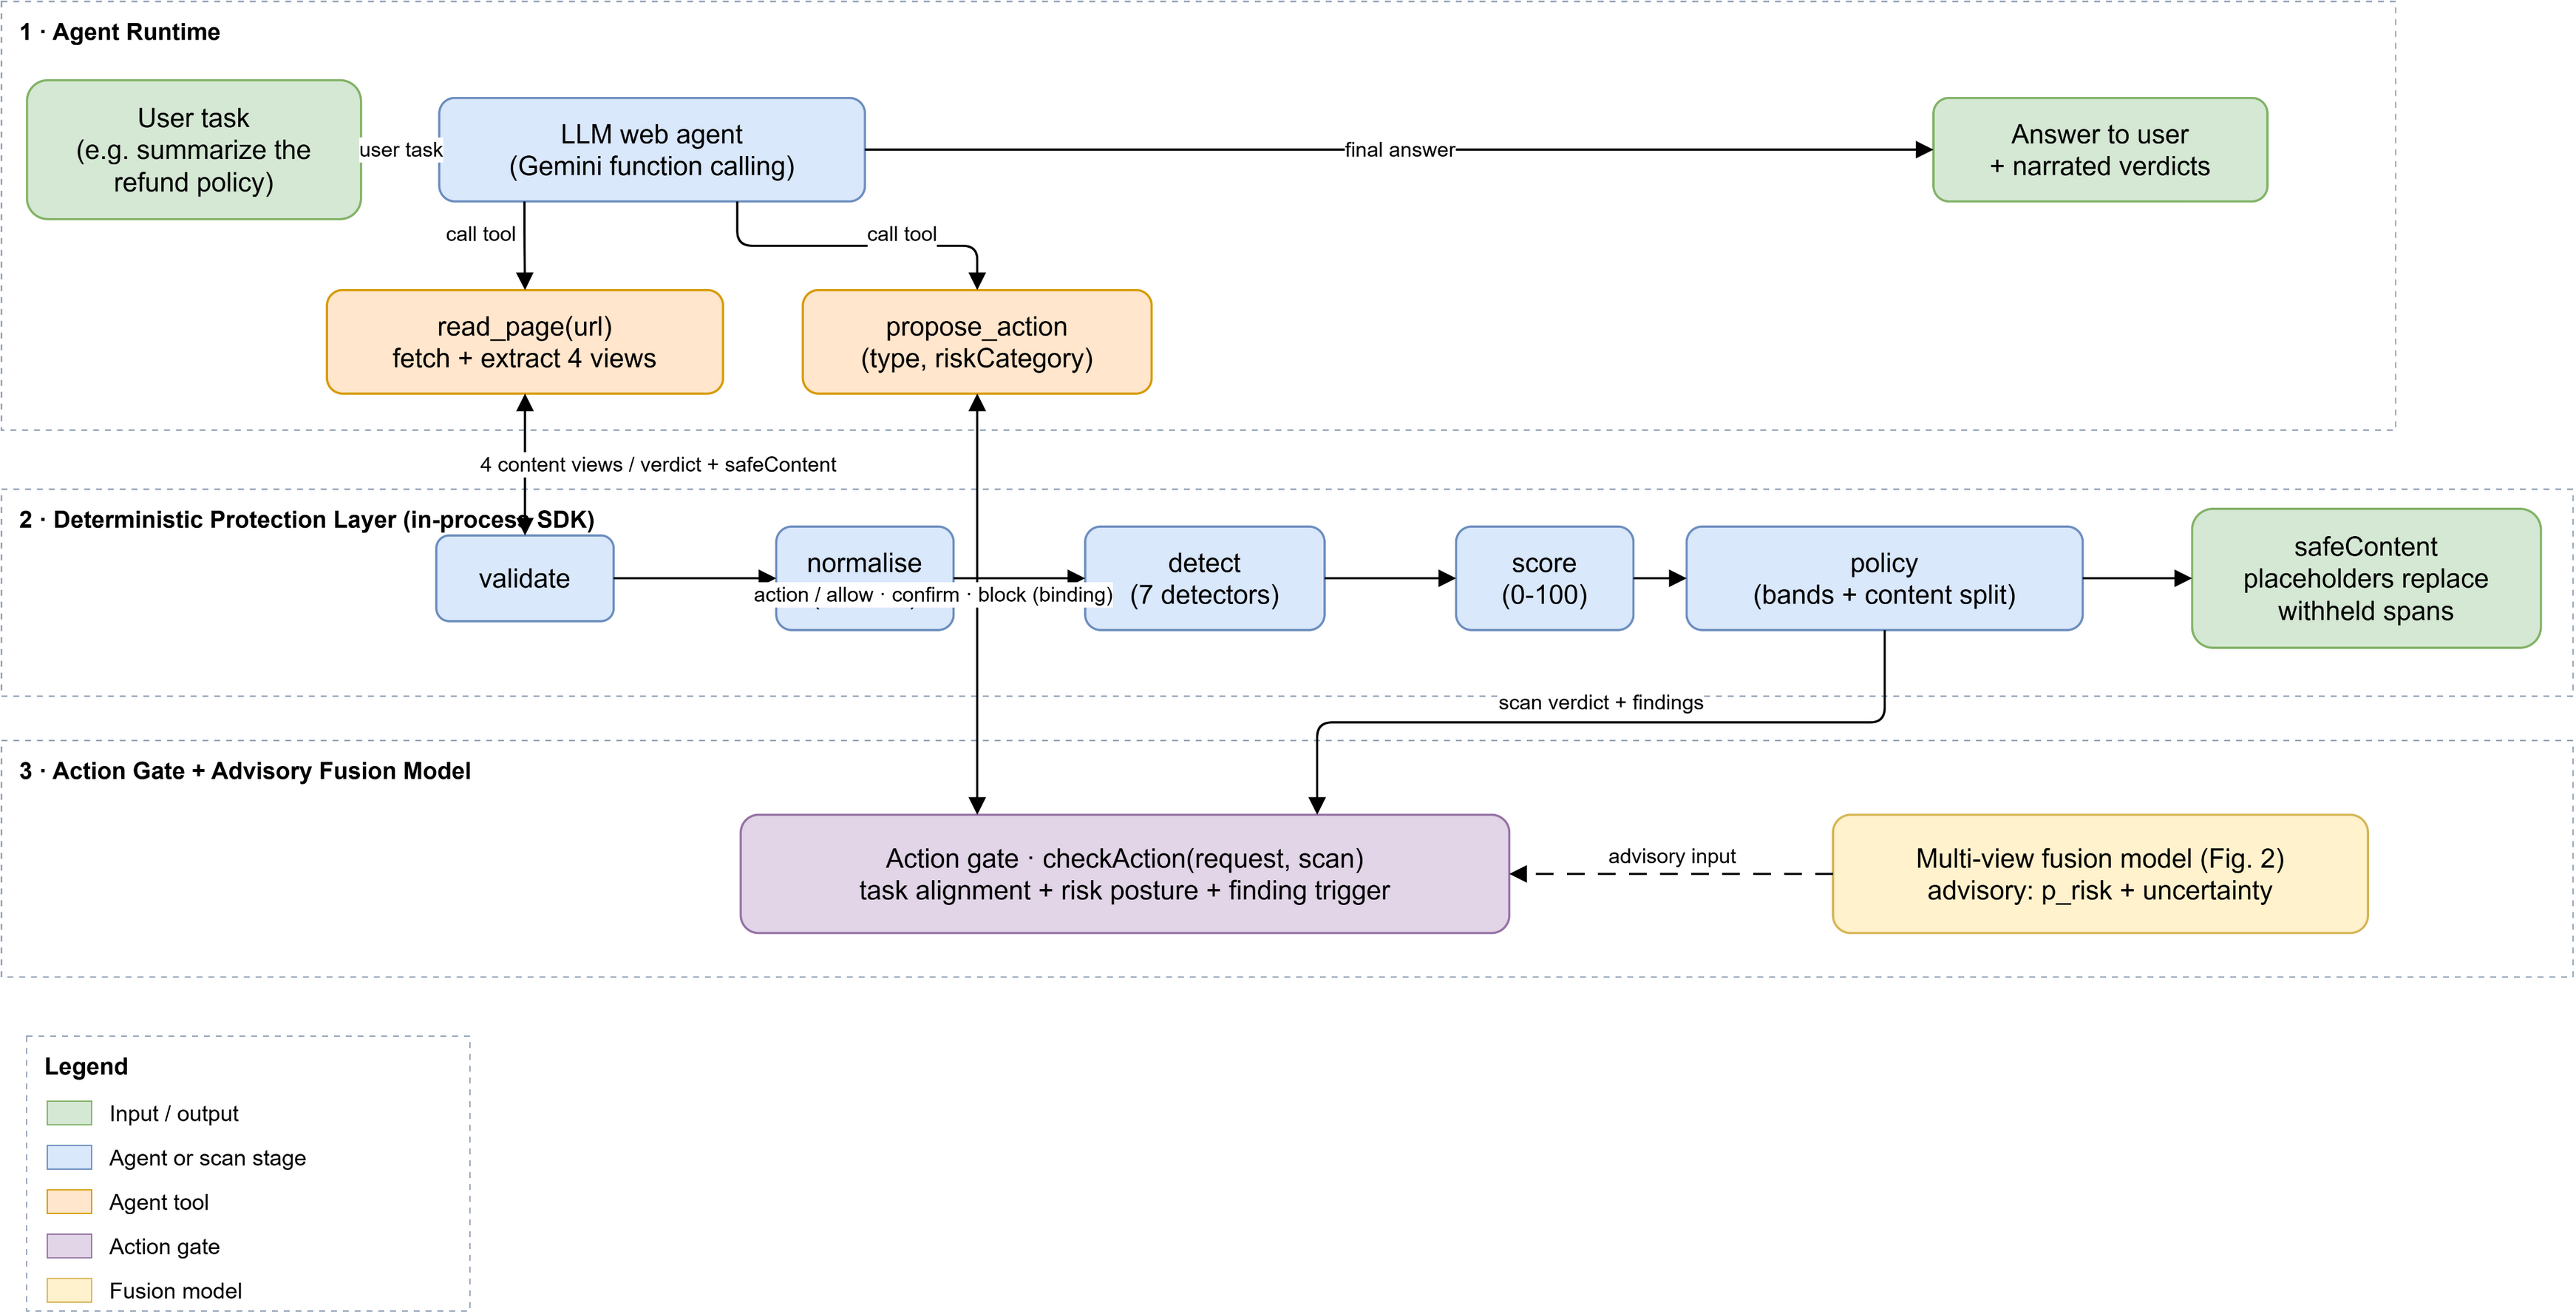
\includegraphics[width=0.98\textwidth]{fig1_system_overview.png}
\caption{End-to-end application block diagram. The LLM web agent (Gemini)
never touches a page directly: \texttt{read\_page} and \texttt{propose\_action}
route through the in-process CtxVigil layer, which scans every page before the
model sees it and gates every action before it executes. Only approved content
(\texttt{safeContent}, with placeholders where attacks were withheld) reaches
the model; a \texttt{block} scan verdict halts the episode entirely.}
\label{fig:overview}
\end{figure*}

\section{Related Work}
\textbf{Attack surface.} Indirect prompt injection was demonstrated against
LLM-integrated applications by Greshake et al.~\cite{greshake2023}, who showed
that retrieved web content can override the agent's instructions. Perez et
al.~\cite{perez2022} systematised direct prompt attacks, and the InjecAgent
benchmark~\cite{injecagent2024} and BIPIA~\cite{bipia2023} operationalised
indirect injection against tool-integrated agents, providing the scenario
grammar (tool hijacking, data exfiltration, privilege escalation) that our
benchmark and fixture pages reuse. AgentDojo~\cite{agentdojo2024} further showed
that injection success depends on both the payload and the tool environment.

\textbf{Defenses.} Existing countermeasures largely fall into three
families: (i) prompt-level hardening and instruction hierarchy, which is
model-dependent and does not inspect the content itself; (ii) learned binary
classifiers over text, which score a page but neither locate the malicious
span nor prevent the model from reading it; and (iii) agent frameworks with
human confirmation, which do not decide \emph{what} to confirm. CtxVigil
differs in two ways: it makes \emph{containment} the primitive (withheld text
is replaced by placeholders and never enters the model's context), and it
splits the decision into two independent gates---content scanning and action
checking---whose combination catches attacks that either gate alone misses
(for example, a clean page carrying an off-task account change).

\section{Proposed Methodology}
\label{sec:methodology}

\subsection{System Overview}
Fig.~\ref{fig:overview} shows the deployed application. An LLM web agent
(Gemini, via a function-calling loop) exposes exactly two tools:
\texttt{read\_page(url)} and \texttt{propose\_action(type, riskCategory)}.
Both tools route through the CtxVigil SDK, which runs in-process with the
agent host. The agent never receives withheld content, and the gate's
decision on any proposed action is final: on a \texttt{block} scan verdict the
episode is halted by the loop itself, so no tool output produced from a
blocked page can reach the user. The same SDK is reachable through three
transports---a CLI, an optional thin HTTP adapter, and an in-process library
call---and all verdicts are rendered in a React dashboard for the
demonstration.

\begin{figure*}[t]
\centering
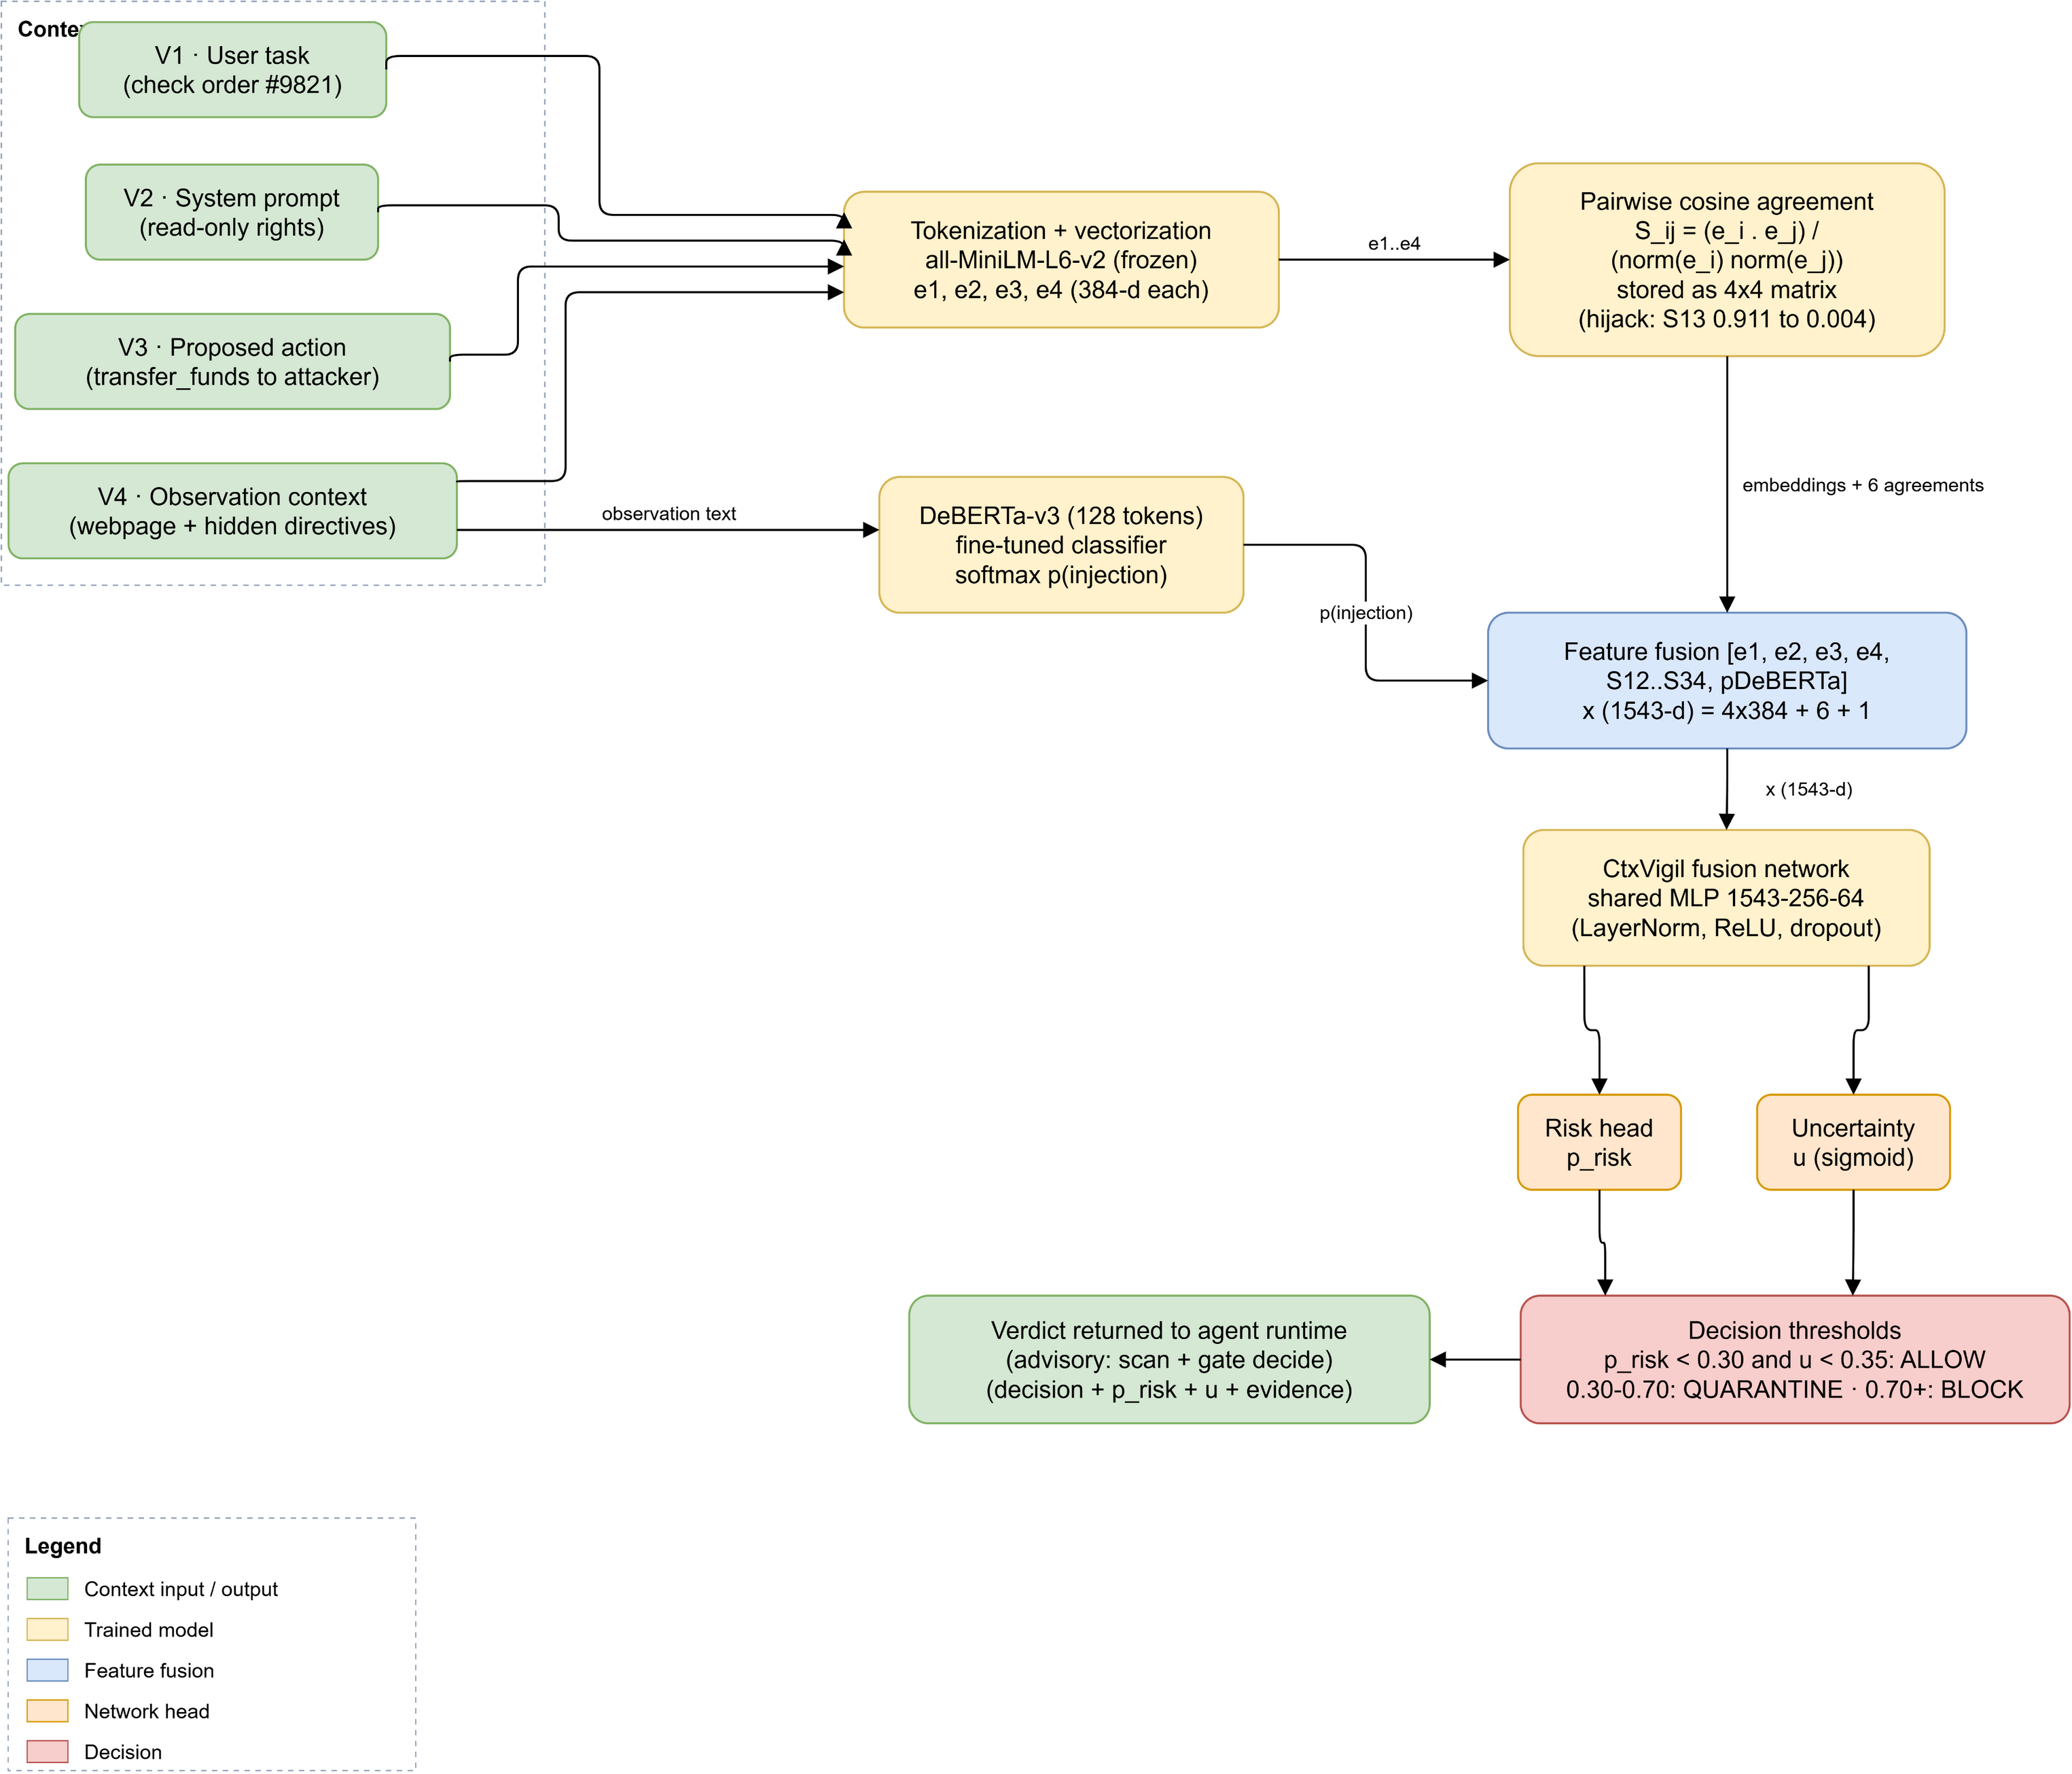
\includegraphics[width=0.98\textwidth]{fig2_layer_architecture.png}
\caption{Detailed architecture of the protection layer. (A) The scan
pipeline: a page is validated and normalised into four content views
(plus a reserved OCR channel), scanned by seven deterministic detectors,
weighted into a 0--100 risk score, and mapped by fixed score bands to a
verdict with per-segment content outputs. (B) The action gate consumes the
proposed action and the scan evidence and returns an independent decision.
(C) The multi-view fusion network (advisory) embeds four agent-context views
with all-MiniLM-L6-v2, augments them with six pairwise cosine agreements and
the DeBERTa injection probability, and produces a risk probability plus an
epistemic uncertainty estimate.}
\label{fig:layer}
\end{figure*}

\subsection{Scan Pipeline}
Fig.~\ref{fig:layer}(A) shows the scan pipeline, executed in five pure,
order-fixed stages:

\subsubsection{Validation and normalisation}
A \texttt{ScanPageRequest} carries the user's task and a page representation
with four content views: visible text, rendered DOM, hidden DOM (elements
with \texttt{display:none} and HTML comments), and the accessibility tree
(ARIA labels and roles), plus a reserved \texttt{image\_text} channel for OCR.
Normalisation produces ordered text segments, each tagged with its view, an
approximate DOM selector, a source kind, and a \emph{concealment} flag
(rendered vs.\ hidden). Provenance is preserved end-to-end: every downstream
finding cites the segment it came from.

\subsubsection{Detection}
Seven deterministic detectors run over the segments and the task text:
\emph{instruction override} (``ignore previous instructions''-style
directives), \emph{role impersonation} (``system notice'', ``admin
authorization''), \emph{data exfiltration} (token-bearing URLs, webhook
addresses), \emph{risky action} (fund transfers, credential changes),
\emph{hidden content} (injections that only appear in concealed channels),
\emph{multi-view repetition} (the same directive repeated across independent
views---a strong injection signature), and \emph{task conflict} (a directive
that contradicts the user's stated task). Each detector emits a finding with
view, selector, signals, severity, and a positive score contribution. All
phrase tables and weights live in a single configuration table; no rule is
inlined in code, and no fixture string is special-cased.

\subsubsection{Scoring and policy}
Category weights aggregate finding contributions into a risk score
\begin{equation}
R \;=\; \min\Bigl(100,\;\sum_{f \in F} w_{c(f)}\cdot s_f \cdot \delta_f\Bigr),
\label{eq:score}
\end{equation}
where $F$ is the finding set, $c(f)$ the risk category of finding $f$,
$w_{c}$ the category weight, $s_f$ the severity multiplier, and
$\delta_f \in [0,1]$ a damping factor that discounts findings whose text is
well-aligned with the user's task vocabulary. A fixed band table maps $R$ to
the verdict: 0--29 \texttt{allow}, 30--59 \texttt{sanitize}, 60--79
\texttt{confirm}, 80--100 \texttt{block}. The policy stage then partitions
content into \texttt{safeContent} (approved segments), 
\texttt{sanitizedContent} (with placeholder markers such as
``\texttt{[Blocked suspicious instruction from aria-label]}''), and
\texttt{blockedContent} (withheld, never delivered to the agent). The
response also carries a plain-English summary that names the deciding
finding---explainability is part of the interface contract, not an
afterthought.

\subsection{Action Gate}
Fig.~\ref{fig:layer}(B) shows the gate, an \emph{independent} decision, never
a re-run of the scan. For a proposed action it evaluates three axes:
(i) \emph{task alignment}---token overlap between the action label and the
user's task, so ``summarize\_policy'' serves ``summarize the refund policy''
while ``change\_account\_email'' does not; (ii) \emph{risk-category posture}---
each category (e.g.\ \texttt{account\_change}, \texttt{data\_transfer},
\texttt{form\_submit}) has an allow/confirm/block posture under the current
configuration; and (iii) \emph{finding triggers}---if a scan exists and a
finding references the action, or if the scan ended in \texttt{block}, the
gate forces a block regardless of alignment. This split catches the case a
content-only filter cannot: a page that reads as benign but still proposes an
unrelated high-risk action.

\subsection{Multi-View Fusion and Uncertainty Network}
\label{sec:fusion}
The learned component, Fig.~\ref{fig:layer}(C), treats an agent checkpoint as
four semantic views: the user task $V_1$, the system prompt $V_2$, the
proposed tool action $V_3$, and the observation context $V_4$. Each view is
embedded with all-MiniLM-L6-v2~\cite{reimers2019} ($e_i \in
\mathbb{R}^{384}$), and pairwise agreement is the cosine similarity
\begin{equation}
S_{ij} \;=\; \frac{e_i^{\!\top} e_j}{\lVert e_i\rVert\,\lVert e_j\rVert},
\qquad i<j \in \{1,\dots,4\},
\label{eq:cosine}
\end{equation}
yielding six agreement features. The task--action agreement $S_{13}$ is the
central hijack signal: an injected observation that steers the agent into
\texttt{transfer\_funds} collapses $S_{13}$ while benign episodes keep
$S_{13}\gg 0.70$. The 1{,}543-dimensional input
($4\times384$ embeddings $+\,6$ agreements $+\,1$ DeBERTa injection
probability from the Stage-1 classifier) feeds a shared MLP encoder
($1543\!\to\!256\!\to\!64$, LayerNorm, ReLU, dropout 0.2) with two heads: a
softmax \emph{risk head} and a sigmoid \emph{epistemic uncertainty head}.
Training minimises the dual objective
\begin{equation}
\mathcal{L} \;=\; \mathcal{L}_{\mathrm{CE}}(y_{\mathrm{risk}}) \;+\;
0.5\,\mathcal{L}_{\mathrm{MSE}}(u),
\label{eq:loss}
\end{equation}
so the model must both classify risk and report calibrated uncertainty;
ambiguous cross-view situations are routed to human confirmation rather than
silently forced either way. In the deployment the fusion output is
\emph{advisory}: the scan and the action gate remain the decisions of record,
so the learned model can never weaken the deterministic guarantees.

\section{Dataset and Preprocessing}
\label{sec:dataset}

\subsection{Benchmark for the Injection Classifier}
The Stage-1 classifier is trained on a 20{,}000-sample benchmark, balanced
between 10{,}000 injection samples and 10{,}000 benign and hard-negative
samples (Table~\ref{tab:dataset}). Injection samples are drawn from 25
curated templates organised into six families that follow the InjecAgent and
BIPIA scenario grammars: direct overrides; indirect context injection
embedded in plausible page furniture (delivery notes, reviews, invoices);
markdown/image exfiltration beacons; jailbreak and roleplay impersonation;
tool manipulation with privilege escalation; and ARIA/DOM cloaking
(\texttt{aria-label} payloads and \texttt{display:none} spans). Each template
is additionally wrapped with randomized contexts so the classifier cannot
memorise exact strings. The benign half draws from 21 templates and
deliberately includes \emph{hard negatives}: system commands, refund
requests, ordinary UI markup with ARIA labels, and sentences that use trigger
words (``ignore'', ``override'', ``system'') in legitimate, non-adversarial
contexts, forcing the classifier to read intent rather than keywords.

\begin{table}[t]
\centering
\caption{Benchmark composition (Stage-1 classifier). Samples are drawn
uniformly at random from the templates of each class.}
\label{tab:dataset}
\begin{tabular}{@{}lrr@{}}
\toprule
\textbf{Class} & \textbf{Templates} & \textbf{Samples} \\
\midrule
Injection (6 families) & 25 & 10{,}000 \\
Benign \& hard negatives & 21 & 10{,}000 \\
\midrule
\textbf{Total} & \textbf{46} & \textbf{20{,}000} \\
\bottomrule
\end{tabular}
\end{table}

Samples are split 70/15/15 (train 14{,}000, validation 3{,}000, test 3{,}000)
with stratification and a fixed seed. Text is tokenised with the DeBERTa-v3
tokenizer, truncated and padded to 128 tokens; no lemmatisation or stopword
removal is applied, since punctuation and markup (e.g.\ markdown image beacons)
are themselves discriminative.

\subsection{Multi-View Episode Dataset}
The fusion network is trained on 5{,}000 synthetic agent episodes, each a
complete 4-tuple $(V_1,V_2,V_3,V_4)$ assembled from realistic task, system,
tool, and observation pools. Episodes are labelled by construction: benign
episodes keep $V_3$ strictly aligned with $V_1$ and $V_2$ with clean
observations ($S_{13}\gg0.70$); injection episodes embed a directive in $V_4$
that hijacks the action (e.g.\ an unauthorised \texttt{transfer\_funds}),
collapsing $S_{13}$; ambiguous episodes add boundary cases with target
uncertainty $u>0.40$. The dataset is split 80/20 into 4{,}000 training and
1{,}000 hold-out episodes. Preprocessing is deterministic: each view is
encoded once with the frozen MiniLM backbone, agreements are computed with
(\ref{eq:cosine}), and the Stage-1 probability is attached as an auxiliary
feature.

\subsection{Fixture Pages for the Deployed Layer}
The rule-based layer is evaluated on six hand-crafted HTML fixture pages
hosted locally (plus two action-check fixtures), covering: a safe refund page
(clean baseline); a visible-text injection; a hidden ARIA-label injection
invisible to a sighted reviewer; a four-channel indirect hijack (ARIA pill +
visible directive + HTML comment + \texttt{display:none} span) modelled on
InjecAgent; a task-deviation page whose directive scans clean but whose
account-change action must be gate-blocked; and a benign hard negative with an
imperative accessible name on a real control. Each page declares its episode
metadata (task, proposed action, expected verdict) in machine-readable
\texttt{ctxvigil:*} meta tags, making the live demo self-checking: a page
whose engine verdict drifts from its declared expectation fails loudly.

\section{Implementation}
\label{sec:implementation}

\subsection{SDK and Transports}
The product is a TypeScript monorepo. The core package
(\texttt{ctxvigil-core}, published as \texttt{ctxvigil} on npm) implements
the five-stage scan pipeline and the action gate with no runtime
dependencies; configuration (phrase tables, weights, postures, thresholds) is
a single JSON-mergeable table so institutions can tune policy without
touching code. Two adapters sit on the same core---a CLI that reads and
writes contract-exact JSON, and an optional thin HTTP adapter---so a verdict
reached through any transport is byte-identical (a parity test asserts this).
The pipeline stages are pure functions, which makes the 145-test suite
(including seven contract fixtures asserted against a normative expectations
file) fast and deterministic.

\subsection{Agent Integration and Demonstration Surfaces}
Two applications demonstrate the layer with a real LLM. The agent chat apps
(terminal CLI and browser chat over an NDJSON event stream) wrap a Gemini
agent whose two tools are the layer's chokepoints; every scan and gate
verdict is narrated live. A deterministic local runner (\texttt{agent:demo})
replays the six fixture pages offline through the same SDK and asserts each
declared verdict, writing a machine-readable run record for the dashboard. The
React dashboard renders the full evidence: per-view page panes, findings with
selectors and signals, the verdict gauge, the action-gate outcome, the agent
trace, and the multi-view agreement inspector.

\subsection{Model Training}
The DeBERTa-v3-small classifier~\cite{he2021,debertav3} was fine-tuned on
Google Colab (T4 GPU) for 3 epochs with the Hugging
Face~\cite{wolf2020} \texttt{Trainer}: batch size 32, learning rate
$2\times10^{-5}$, weight decay 0.01, sequences of 128 tokens, fixed seed. The
fusion network~(\ref{sec:fusion}) is a compact PyTorch~\cite{paszke2019} MLP
trained for 15 epochs with AdamW (learning rate $10^{-3}$, weight decay
$10^{-4}$, batch 64) under the joint objective~(\ref{eq:loss}). Model weights,
test inferences, and a metrics summary are exported for reproducibility, and
both training pipelines are published as Kaggle/Colab notebooks in the
repository.

\section{Experimentation and Results}
\label{sec:results}

\subsection{Stage-1 Classifier}
On the 3{,}000-sample held-out test set the fine-tuned DeBERTa-v3-small
classifier achieves 100.00\% accuracy, 100.00\% precision, 100.00\% recall,
100.00\% F1, and ROC-AUC 1.000 (Table~\ref{tab:deberta}). The exported
test-inference sample (500 rows: 243 injections, 257 benign) shows the same
perfect separation: the confusion matrix (Fig.~\ref{fig:cm}) has zero
off-diagonal entries, the ROC curve hugs the axes (Fig.~\ref{fig:roc}), and
the predicted-probability histogram (Fig.~\ref{fig:sep}) shows two spikes at
0.0 and 1.0 with no mass in between. The hard negatives---benign sentences
containing ``ignore'' and ``override''---are classified correctly, confirming
that the model reacts to structure and intent rather than keywords alone.

\begin{table}[t]
\centering
\caption{DeBERTa-v3-small on the 3{,}000-sample held-out test set.}
\label{tab:deberta}
\begin{tabular}{@{}lr@{}}
\toprule
\textbf{Metric} & \textbf{Value} \\
\midrule
Accuracy & 100.00\% \\
Precision & 100.00\% \\
Recall & 100.00\% \\
F1-score & 100.00\% \\
ROC-AUC & 1.000 \\
\bottomrule
\end{tabular}
\end{table}

\begin{figure}[t]
\centering
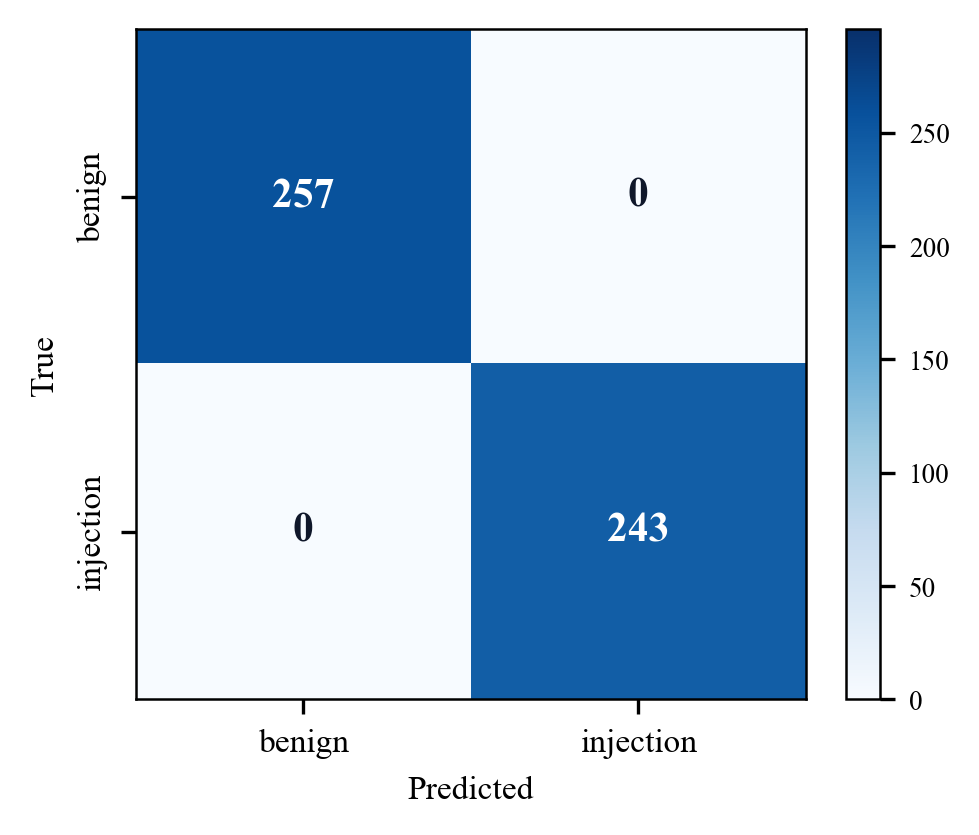
\includegraphics[width=0.85\columnwidth]{fig3_confusion_matrix.png}
\caption{Confusion matrix on the exported test-inference sample
(243 injection, 257 benign): zero false positives and zero false negatives.}
\label{fig:cm}
\end{figure}

\begin{figure}[t]
\centering
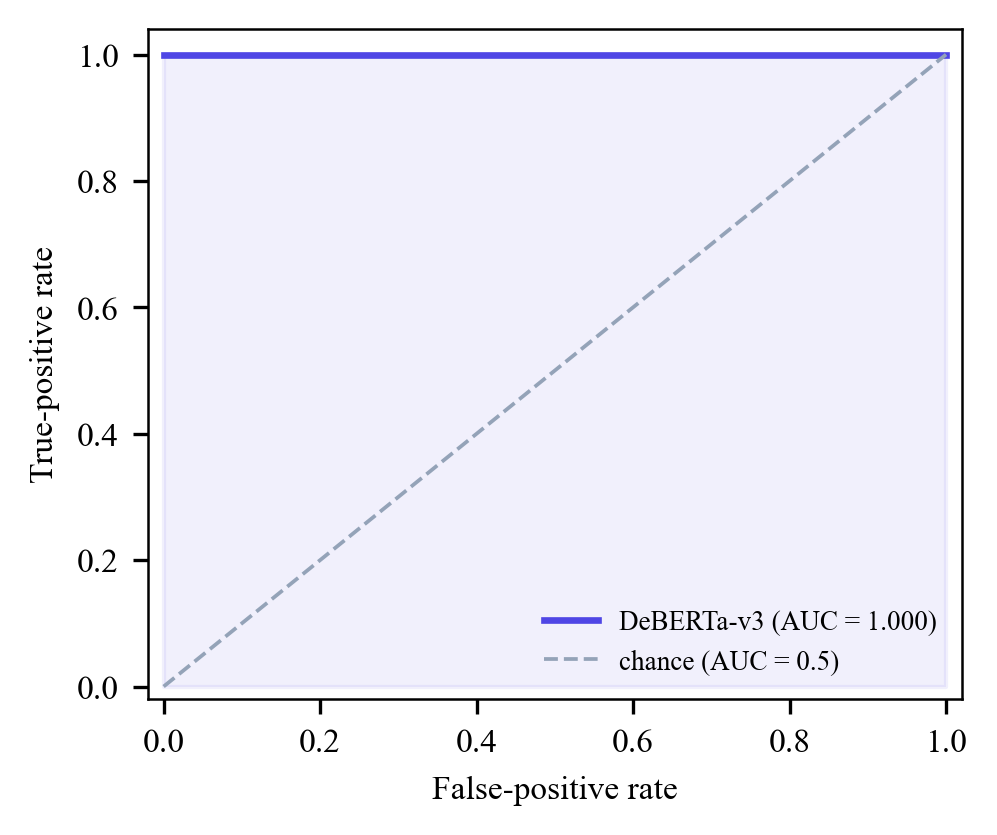
\includegraphics[width=0.85\columnwidth]{fig4_roc.png}
\caption{ROC curve of the Stage-1 classifier on the exported sample
(AUC $=1.000$).}
\label{fig:roc}
\end{figure}

\begin{figure}[t]
\centering
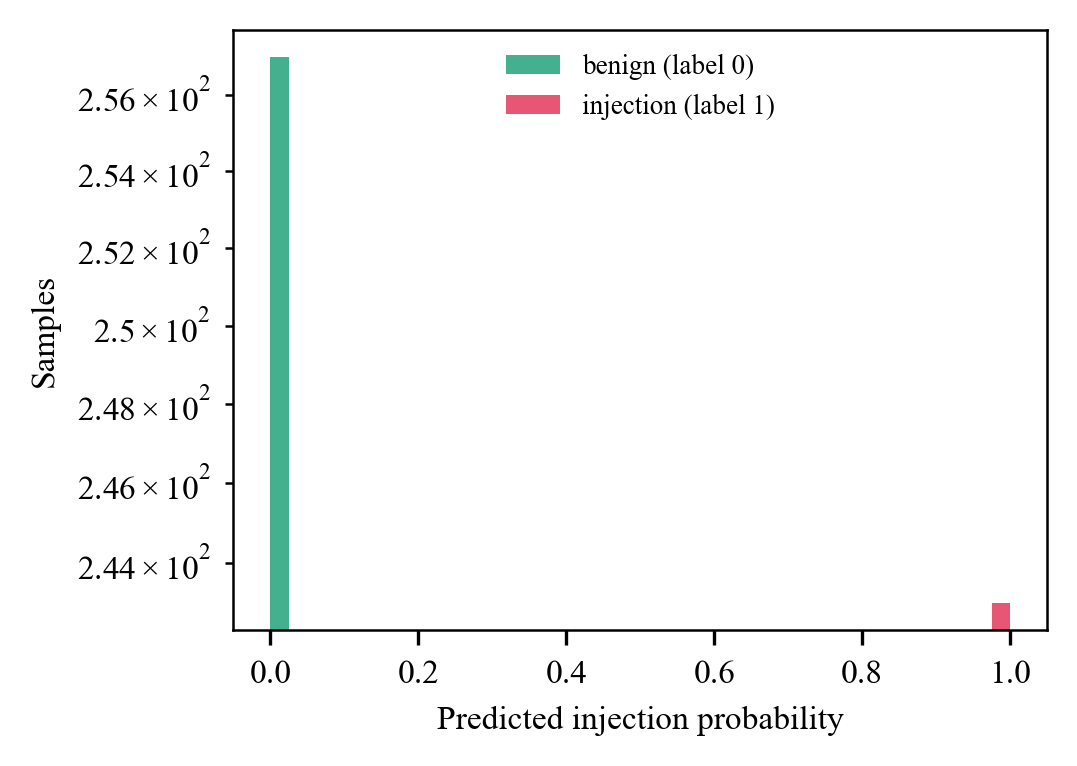
\includegraphics[width=0.95\columnwidth]{fig5_prob_separation.png}
\caption{Predicted-probability separation between benign and injection
samples (log scale): the model assigns saturating probabilities with no
decision-boundary mass.}
\label{fig:sep}
\end{figure}

\subsection{Multi-View Fusion Network}
\label{sec:results-ml}
On the 1{,}000-episode hold-out set the fusion network reaches 100\%
accuracy, precision, recall, and F1, with ROC-AUC 1.000
(Table~\ref{tab:fusion}). More informative than the headline numbers is the
behaviour of the uncertainty head: benign episodes receive low uncertainty,
hijacked episodes are driven by the collapse of the task--action agreement
$S_{13}$, and ambiguous boundary episodes---deliberately included in the
episode pool---collect elevated uncertainty, which routes them to human
confirmation under the gate thresholds (risk $<0.30$ and uncertainty
$<0.35$ $\Rightarrow$ \texttt{ALLOW}; risk $\geq0.70$ $\Rightarrow$
\texttt{BLOCK}; otherwise \texttt{QUARANTINE}/confirm). The live simulation in
the notebook confirms the two canonical scenarios: a benign order-status
query is allowed, while an InjecAgent-style hijack
(\texttt{transfer\_funds} to an attacker wallet under an injected directive,
with $p_{\mathrm{DeBERTa}}=0.98$) is blocked.

\begin{table}[t]
\centering
\caption{Fusion network on 1{,}000 hold-out episodes.}
\label{tab:fusion}
\begin{tabular}{@{}lr@{}}
\toprule
\textbf{Metric} & \textbf{Value} \\
\midrule
Risk accuracy & 100\% \\
Precision / Recall & 100\% / 100\% \\
F1-score & 100\% \\
ROC-AUC & 1.000 \\
Model size & 1.6\,MB (MLP weights) \\
\bottomrule
\end{tabular}
\end{table}

\subsection{Rule-Based Layer: Contract Fixtures}
The deployed layer is evaluated against seven normative fixtures with a
declared expected verdict each. All seven assertions pass
(Table~\ref{tab:fixtures} and Fig.~\ref{fig:rule}). Three results deserve
emphasis. First, the \emph{hidden ARIA injection} scores 100 (\texttt{block})
although nothing visible on the rendered page is suspicious---the payload
lives in a support button's accessible name and is caught only because the
accessibility tree is scanned as a first-class view. Second, the
\emph{four-channel hijack} page accumulates five findings across ARIA,
visible, hidden-DOM, and comment channels, demonstrating cross-view
corroboration (the multi-view repetition detector fires because the same
directive appears in several channels). Third, the \emph{benign hard
negative} scores 0 (\texttt{allow}) despite an imperative accessible name on
its submit control, and the \emph{unrelated account action} scans clean but
is gate-blocked---together demonstrating that the layer neither
over-blocks ordinary pages nor relies on the scan alone.

\begin{table}[t]
\centering
\caption{Observed verdicts on the seven contract fixtures (rule layer).}
\label{tab:fixtures}
\begin{tabular}{@{}lrlr@{}}
\toprule
\textbf{Fixture} & \textbf{Score} & \textbf{Scan} & \textbf{Gate} \\
\midrule
safe-refund-page & 0 & allow & allow \\
visible-injection & 65 & confirm & confirm \\
hidden-dom-injection & 95 & block & block \\
aria-injection & 100 & block & block \\
benign-aria-label & 0 & allow & allow \\
unrelated-account-action & 0 & allow & \textbf{block} \\
task-aligned-summary-action & 0 & allow & allow \\
\bottomrule
\end{tabular}
\end{table}

\begin{figure}[t]
\centering
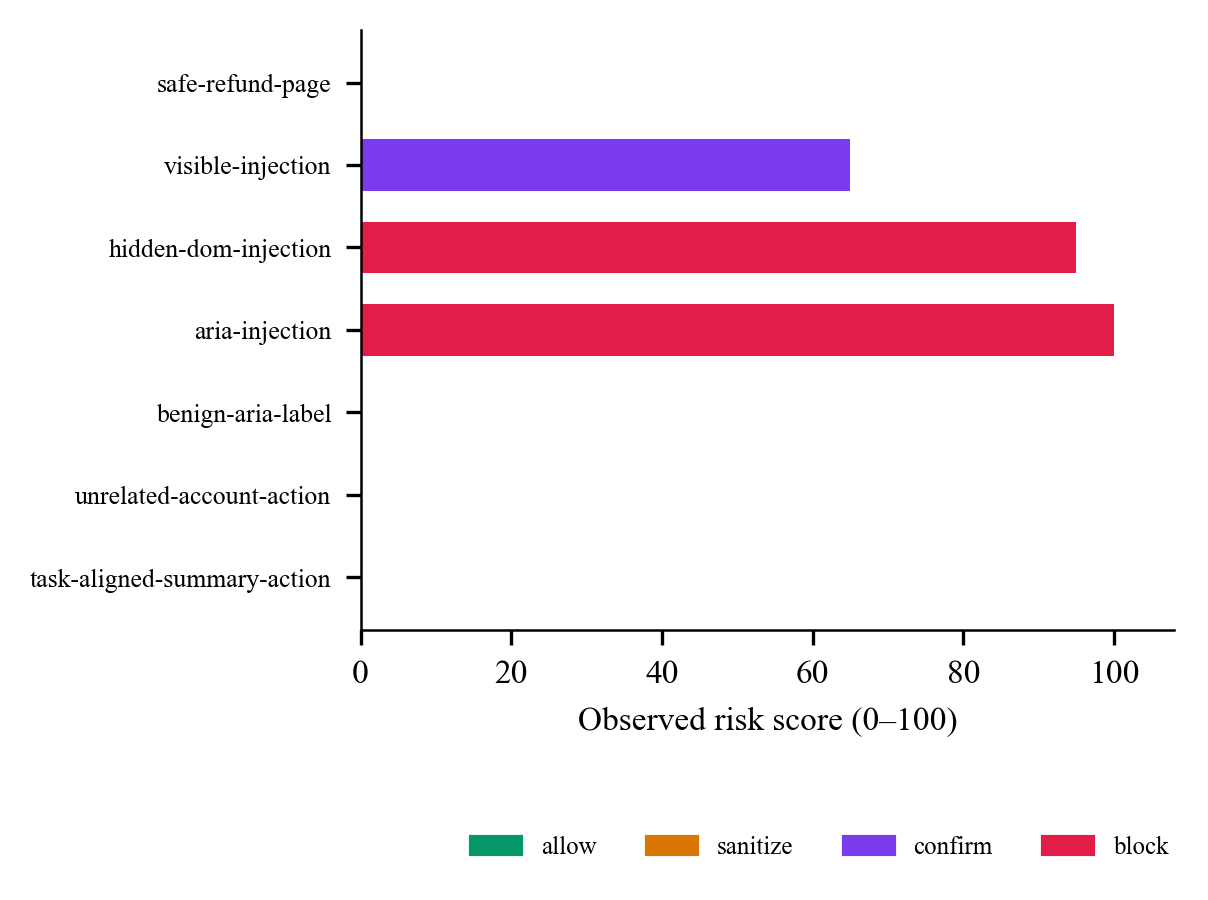
\includegraphics[width=0.95\columnwidth]{fig6_rule_layer_scores.png}
\caption{Observed risk scores and verdicts across the seven contract
fixtures, coloured by decision.}
\label{fig:rule}
\end{figure}

\subsection{Live Agent Episodes and Latency}
A scripted agent replays all six fixture pages through the real SDK over
HTTP; all six declared verdicts assert correctly (two blocks, one
escalation, three allows), with per-episode end-to-end latency of
2--21\,ms on a commodity laptop CPU (Table~\ref{tab:latency})---fully
offline, no GPU and no model API involved in the rule path. For
comparison, the LLM-driven chat demo adds Gemini round-trips on top of the
same layer, which is why the deterministic path remains the
default enforcement: it adds negligible overhead to the agent loop while
providing the containment guarantee.

\begin{table}[t]
\centering
\caption{Per-episode latency of the live agent runner (CPU, offline).}
\label{tab:latency}
\begin{tabular}{@{}lrr@{}}
\toprule
\textbf{Episode} & \textbf{Latency (ms)} & \textbf{Gate} \\
\midrule
aria-injection & 21 & block \\
injecagent-indirect-hijack & 3 & block \\
visible-injection & 2 & confirm \\
task-deviation-settings & 3 & block \\
benign-aria-negative & 2 & allow \\
safe-refund-page & 2 & allow \\
\midrule
\textbf{All six episodes} & \textbf{33} & 6/6 pass \\
\bottomrule
\end{tabular}
\end{table}

\subsection{Discussion and Limitations}
The perfect classifier and fusion scores must be read in context: the
benchmark and episode datasets are template-derived, so the learned models
demonstrate achievable separation on the attack families they were designed
around, not robustness to arbitrary novel injections. The deployment
consequently treats the learned components as \emph{advisory} signals and
keeps enforcement in the deterministic, explainable path, whose behaviour is
asserted by contract tests rather than by held-out accuracy. The rule layer
has its own limits---phrase tables must be maintained, and a semantically
novel phrasing outside the seven detectors is caught by the gate's
alignment/posture axes rather than by the scan. Combining the two---using
the fusion network's risk and uncertainty as a learned calibrator behind the
same policy interface---is the natural next step, together with evaluation
on external benchmarks such as the full InjecAgent and AgentDojo suites.

\section{Conclusion}
CtxVigil demonstrates that protection for LLM web agents can be explainable,
fast, and fail-closed without sacrificing usability. Its multi-view scan
pipeline catches injections that are invisible to both sighted reviewers and
single-view filters, its independent action gate blocks off-task actions on
pages that scan clean, and its learned fusion network quantifies cross-view
disagreement with calibrated uncertainty---while a real Gemini agent,
wrapped by the layer, narrates every verdict live at 2--21\,ms per episode
on a commodity CPU. All code, notebooks, fixtures, test suites, and
evaluation artifacts are available in the project repository at
\texttt{github.com/rishabhx29/Prompt-Injection-Detection-Model}.

\begin{thebibliography}{9}

\bibitem{greshake2023}
K.~Greshake et al., ``Not what you've signed up for: Compromising real-world
LLM-integrated applications with indirectly prompt injection,'' in \emph{Proc.
16th ACM Workshop on Artificial Intelligence and Security (AISec)}, 2023,
pp. 79--90.

\bibitem{injecagent2024}
Q.~Zhan et al., ``InjecAgent: Benchmarking indirect prompt injections in
tool-integrated large language model agents,'' \emph{arXiv:2403.02691}, 2024.

\bibitem{bipia2023}
F.~Yi et al., ``Benchmarking and defending against indirect prompt injection
attacks on large language models,'' \emph{arXiv:2312.14197}, 2023.

\bibitem{agentdojo2024}
E.~Debenedetti et al., ``AgentDojo: A dynamic environment to evaluate
prompt injection attacks and defenses for LLM agents,'' \emph{arXiv:2406.13352},
2024.

\bibitem{perez2022}
F.~Perez et al., ``Ignore previous prompt: Attack techniques for language
models,'' \emph{arXiv:2211.09527}, 2022.

\bibitem{owasp2025}
OWASP Foundation, ``OWASP Top 10 for Large Language Model Applications,''
2025. [Online]. Available: https://genai.owasp.org/

\bibitem{he2021}
P.~He, X.~Liu, J.~Gao, and W.~Chen, ``DeBERTa: Decoding-enhanced BERT with
disentangled attention,'' in \emph{Proc. Int. Conf. on Learning
Representations (ICLR)}, 2021.

\bibitem{debertav3}
P.~He, J.~Gao, and W.~Chen, ``DeBERTaV3: Improving DeBERTa using
ELECTRA-style pre-training with gradient-disentangled embedding sharing,''
\emph{arXiv:2111.09543}, 2021.

\bibitem{reimers2019}
N.~Reimers and I.~Gurevych, ``Sentence-BERT: Sentence embeddings using
Siamese BERT-networks,'' in \emph{Proc. Conf. on Empirical Methods in Natural
Language Processing (EMNLP)}, 2019, pp. 3982--3992.

\bibitem{wolf2020}
T.~Wolf et al., ``Transformers: State-of-the-art natural language
processing,'' in \emph{Proc. Conf. on Empirical Methods in Natural Language
Processing (EMNL): System Demonstrations}, 2020, pp. 38--45.

\bibitem{paszke2019}
A.~Paszke et al., ``PyTorch: An imperative style, high-performance deep
learning library,'' in \emph{Proc. Advances in Neural Information Processing
Systems (NeurIPS)}, vol.~32, 2019.

\bibitem{pedregosa2011}
F.~Pedregosa et al., ``Scikit-learn: Machine learning in Python,'' \emph{J.
Mach. Learn. Res.}, vol.~12, pp. 2825--2830, 2011.

\end{thebibliography}

\end{document}
